\section{Experiments and analysis}


\begin{frame}{Experiments and analysis}
\begin{block}{動画}
640x480, 25fps, 4000fames (2100 forged) from 20 videos 
\end{block}
\begin{block}{改ざん編集}
Mokey 4.1.4\footnote{Scientific \& Engineering Award from The Academy of Motion Pictures https://www.imagineersystems.com}
\includegraphics[height=4cm]{figure/mocha.jpg}
\end{block}
\end{frame}


\begin{frame}\frametitle{Original videos}
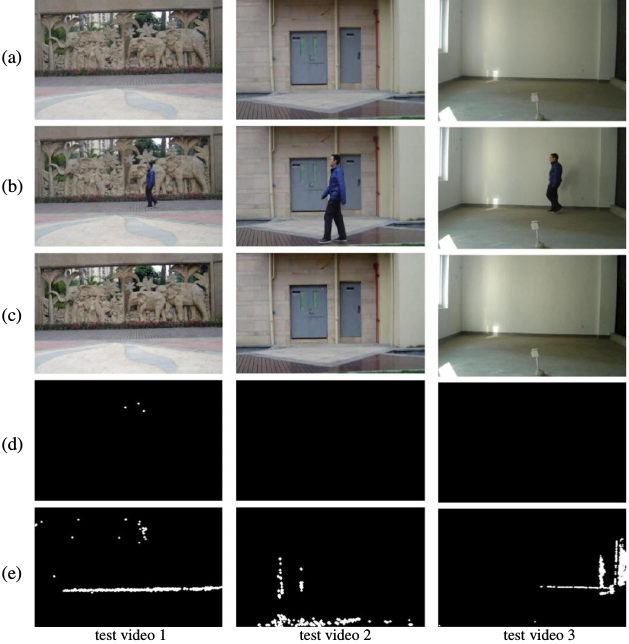
\includegraphics[height=6cm]{figure/result1.png}
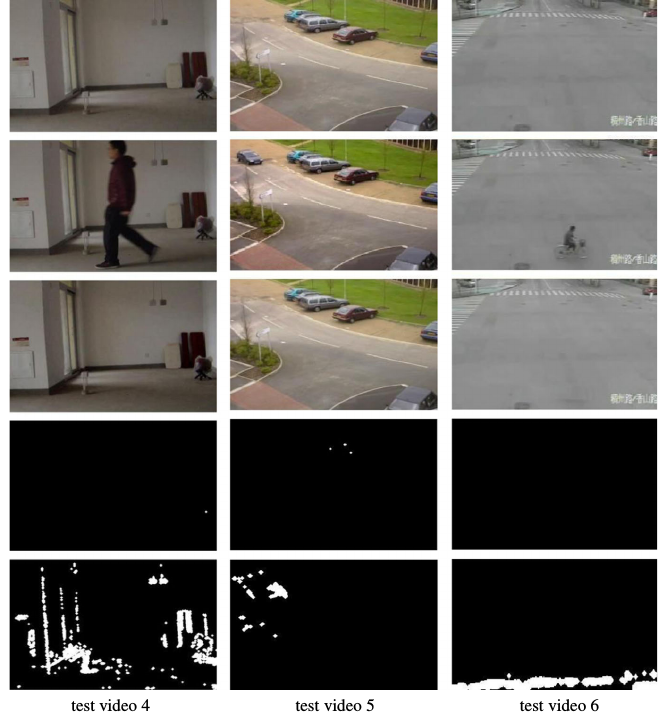
\includegraphics[height=6cm]{figure/result0.png}

(a) 背景 (b) 元映像 (c) 改ざん映像 (d) a の結果 (e) c の結果
\end{frame}


\begin{frame}\frametitle{A downloaded video}
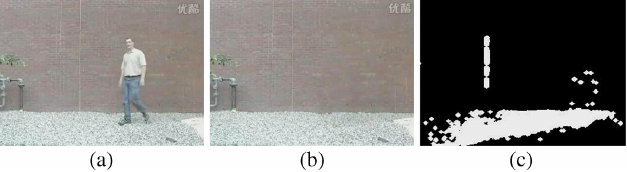
\includegraphics[width=\textwidth]{figure/result2.png}

(a) 元映像 (b) 改ざん映像 (c) 結果
\end{frame}


\begin{frame}\frametitle{Experimental results}
\begin{block}{良かった点}
\begin{itemize}
  \item 背景の検出結果は誤検出が少ない
  \item video 4 は照明が強いのでうまくいった
  \item video 6 の監視カメラ映像でもうまくいった
\end{itemize}
\end{block}
\begin{alertblock}{悪かった点}
\begin{itemize}
  \item video 1 では木の葉がよく誤検出された
  \item DL された動画は再圧縮による悪影響がみられた
\end{itemize}
\end{alertblock}
\end{frame}


\begin{frame}\frametitle{Peformance indices}
K-Means で識別されるが,本来はトレードオフなタスク
\begin{block}{Indices}
T(F): True (False),\; P(N): Positive (Negative) 
\begin{eqnarray}
    Precision \; Rate & = & \frac{TP}{TP + FP} \\
    Recall \; Rate & = & \frac{TP}{TP + FN} \\
    Detection \; Accuracy & = & \frac{TP + TN}{TP + TN + FP + FN}
\end{eqnarray}
\end{block}
\end{frame}


\begin{frame}\frametitle{Comparison with other algorithms}
[Zhang 09]\footnote{Optical-flow に基づく特徴量の閾値による Video-Inpating と Copy-Paste 検出手法 (文献\cite{Zhang2009})} と [Song 11] と比較

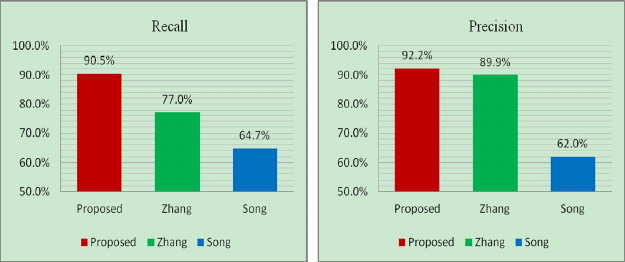
\includegraphics[height=3cm]{figure/recall_prec.png}
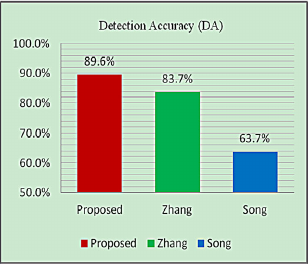
\includegraphics[height=3cm]{figure/accuracy.png}

\begin{itemize}
    \item 良い
\end{itemize}
\end{frame}
